% !TEX root = ../main.tex

%*****************************************
\chapter[Spectroscopic database]{A near-infrared spectroscopic database of high-redshift quasars}
\label{ch:nirsample}
%*****************************************

\section{Spectroscopic surveys}

Emission-lines provide a wealth of information about the properties of AGN and their environments. 
They provide diagnostics of dynamics, temperatures, densities, dust content, elemental abundances and the shape of the ionising spectrum which are often unattainable through any other technique. 
The rest-frame optical region includes a number of strong emission features, including the broad Balmer lines \ha ($6565$\,\AA) and \hb ($4863$\,\AA) and the narrow [\ion{O}{III}]$\lambda\lambda$$4960$,$5008$ doublet.
As we will see in Chapter~\ref{ch:bhmass}, the Balmer lines are routinely used to derive BH masses and AGN accretion rates. 
As the strongest narrow emission-line in the rest-frame optical spectrum, [\ion{O}{III}] is used to measure systemic redshifts, and to probe AGN-driven outflows in the NLR (see Chapter~\ref{ch:nlr}). 

Large optical surveys have provided spectra for hundreds of thousands of AGN and quasars. 
With it's twelfth data release in $2016$, the number of AGN and quasars in the SDSS spectroscopic catalogue alone reached almost $400\,000$. 
However, the rest-frame optical region is redshifted beyond the reach of optical spectrographs at redshifts $z \gtrsim0.4$. 
Accessing the rest-frame optical lines at redshifts $2 \lesssim z \lesssim 4$, during the peak epoch of galaxy evolution, requires near-infrared spectroscopy.  

Spectroscopic observations are more challenging at near-infrared wavelengths than in the optical because the Earth's atmosphere is both bright and highly variable at infrared wavelengths. 
As a result, the number of high-redshift quasars with near-infrared spectra is limited and previous investigations of the rest-frame optical spectra of quasars at redshifts $z\sim2$ have typically used samples containing a few dozen objects \citep[e.g.][]{marziani09,shen12,shen16a}. 

In this chapter, we will describe the construction of a database containing $434$ high-redshift quasars with near-infrared spectra. 
In later chapters, we will describe how this data has been used to significantly reduce large systematic biases afflicting BH mass estimates for quasars at redshifts $z \gtrsim 2$ (Chapter~\ref{ch:bhmass}) and to study the prevalence and drivers of quasar-driven galaxy-wide outflows (Chapter~\ref{ch:nlr}). 
The unprecedented size and quality of this dataset make a number of other investigations possible, some of which are described in Chapter~\ref{ch:summary}. 

\section{Near-infrared spectroscopic data}

\begin{table}
  \footnotesize
  \centering
    \begin{tabular}{cc} 
    \hline
    Instrument & Number \\  
    \hline
    FIRE/Magellan   & $36$ \\
    GNIRS/Gemini    & $29$ \\
    ISAAC/VLT       & $13$  \\
    LIRIS/WHT       & $21$  \\
    NIRI/Gemini     & $31$ \\
    NIRSPEC/Keck    & $3$   \\ 
    SINFONI/VLT     & $84$ \\
    SofI/NTT        & $111$ \\
    TRIPLESPEC/ARC  & $38$ \\
    TRIPLESPEC/Hale & $60$ \\
    XSHOOTER/VLT    & $36$  \\
    \hline
    Total & $462$ \\
    \hline
    \end{tabular}
    \caption[{Number of database objects observed with each near-infrared spectrograph/telescope.}]{Number of database objects observed with each near-infrared spectrograph/telescope.}
  \label{tab:data_summary}
\end{table}

The near-infrared spectra in our database are taken from published catalogues, by downloading and reducing
archival spectra, and by reducing previously un-published spectra acquired in programmes led by Prof. J. Hennawi (UCSB) and Prof. X. Prochaska (UCO/LICK).
We undertook two further observing programmes (Principal Investigator (PI): L. Coatman) to increase the number of objects in under-sampled regions of the \ion{C}{IV} EQW and blueshift parameter space (see Section~\ref{sec:ch3-intro} for a detailed discussion of \ion{C}{IV} emission properties in high-redshift quasars).
The telescopes and instruments used to observe the spectra are summarised in Table~\ref{tab:data_summary} and information on individual spectra is provided in Table~\ref{tab:database}.
There are $434$ unique quasars in our catalogue. 
Multiple spectra exists for a number of quasars, and the total number of spectra in our catalogue is $462$. 
The columns in Table~\ref{tab:database} are as follows: 

\begin{itemize}

\item[1] ID: Jhhmmss+ddmmss. ID is repeated when multiple spectra exist for the same object. 

\item[2] Unique catalogue name.   

\item[3] Date spectrum acquired. 

\item[4-5] RA and DEC (J$2000$; truncated coordinates).  

\item[6] Instrument and telescope used to acquire spectrum. 

\item[7] Wavelength range covered by spectrum. 

\item[8] Velocity per pixel in spectrum. 

\item[9] Signal-to-noise ratio (S/N) per pixel in spectrum. 

\item[10] Redshift. 

\end{itemize}

\begin{landscape}% Landscape page
    \centering % Center table
    \begin{minipage}{\linewidth}
    \footnotesize
    \renewcommand\footnoterule{}
    \captionof{table}[Quasars in the near-infrared spectroscopic database.]{Quasars in the near-infrared spectroscopic database. Only the first $15$ entries are shown. The full table (including $462$ objects) is available online at http://dx.doi.org/10.5281/zenodo.557069.}
    \label{tab:database}
    \begin{tabular}{cccccccccc} 
    \toprule
     ID &   Cat. Name &  Date &             Ra &            Dec &            Instr. &  $\Delta\lambda$ [$\mu$m] &  $\Delta v$ [\kms] & S/N &  $z$ \\
     ($1$) &        ($2$) &             ($3$) &            ($4$) &            ($5$) &  ($6$) &  ($7$) & ($8$) &  ($9$) & ($10$) \\
    \midrule
    J$000039$-$001804$  &  QSO$460$ & $2015$-$09$-$02$ &  +$00$h$00$m$39$.$00$s &  -$00$d$18$m$03$.$90$s &         SofI/NTT &  $1.50$-$2.54$ &     $154.0$ &   $4.9$ &  $2.14$ \\
    J$000345$-$232353$  &  QSO$552$ & $2009$-$07$-$07$ &  +$00$h$03$m$45$.$00$s &  -$23$d$23$m$53$.$40$s &      SINFONI/VLT &  $1.44$-$1.87$ &      $36.0$ &  $12.7$ &  $2.27$ \\
    J$000345$-$232353$  &  QSO$330$ & $2011$-$09$-$18$ &  +$00$h$03$m$45$.$00$s &  -$23$d$23$m$53$.$40$s &         SofI/NTT &  $1.48$-$1.83$ &      $63.0$ &  $36.0$ &  $2.26$ \\
    J$000451$-$084450$  &  QSO$290$ & $2013$-$07$-$12$ &  +$00$h$04$m$50$.$66$s &  -$08$d$44$m$49$.$63$s &     XSHOOTER/VLT &  $0.31$-$2.28$ &      $15.0$ &  $10.3$ &  $3.00$ \\
    J$000451$-$084452$  &  QSO$289$ & $2013$-$08$-$08$ &  +$00$h$04$m$50$.$91$s &  -$08$d$44$m$51$.$98$s &     XSHOOTER/VLT &  $0.31$-$2.28$ &      $15.0$ &   $5.4$ &  $3.00$ \\
    J$000500$-$003348$  &  QSO$454$ & $2015$-$09$-$01$ &  +$00$h$05$m$00$.$42$s &  -$00$d$33$m$48$.$20$s &         SofI/NTT &  $1.50$-$2.54$ &     $154.0$ &   $8.2$ &  $2.18$ \\
    J$000501$+$010221$  &  QSO$459$ & $2015$-$09$-$02$ &  +$00$h$05$m$00$.$53$s &  +$01$d$02$m$20$.$80$s &         SofI/NTT &  $1.50$-$2.54$ &     $154.0$ &   $6.8$ &  $2.13$ \\
    J$001016$+$001228$  &  QSO$475$ & $2015$-$09$-$04$ &  +$00$h$10$m$16$.$49$s &  +$00$d$12$m$27$.$60$s &         SofI/NTT &  $1.50$-$2.54$ &     $154.0$ &   $8.9$ &  $2.28$ \\
    J$001247$+$001239$  &  QSO$082$ & $2013$-$06$-$06$ &  +$00$h$12$m$47$.$12$s &  +$00$d$12$m$39$.$49$s &        ISAAC/VLT &  $1.52$-$1.60$ &      $15.0$ &  $19.1$ &  $2.16$ \\
    J$001708$+$813508$  &  QSO$107$ & $2012$-$08$-$04$ &  +$00$h$17$m$08$.$48$s &  +$81$d$35$m$08$.$10$s &  TRIPLESPEC/Hale &  $0.94$-$2.80$ &      $39.0$ &  $36.5$ &  $3.40$ \\
    J$001919$+$010152$  &  QSO$476$ & $2015$-$09$-$04$ &  +$00$h$19$m$19$.$31$s &  +$01$d$01$m$52$.$20$s &         SofI/NTT &  $1.50$-$2.54$ &     $154.0$ &   $6.5$ &  $2.32$ \\
    J$001955$-$091316$  &  QSO$001$ & $2004$-$11$-$26$ &  +$00$h$19$m$54$.$67$s &  -$09$d$13$m$16$.$45$s &     GNIRS/Gemini &  $0.60$-$2.61$ &      $88.0$ &   $9.9$ &  $2.12$ \\
    J$002018$-$233654$  &  QSO$553$ & $2009$-$07$-$07$ &  +$00$h$20$m$18$.$41$s &  -$23$d$36$m$53$.$80$s &      SINFONI/VLT &  $1.44$-$1.87$ &      $36.0$ &  $16.9$ &  $2.30$ \\
    J$002023$-$414639$  &  QSO$554$ & $2009$-$07$-$08$ &  +$00$h$20$m$23$.$38$s &  -$41$d$46$m$38$.$90$s &      SINFONI/VLT &  $1.09$-$1.41$ &      $35.0$ &  $33.4$ &  $1.57$ \\
    J$002111$-$242247$  &  QSO$555$ & $2009$-$07$-$16$ &  +$00$h$21$m$10$.$90$s &  -$24$d$22$m$47$.$20$s &      SINFONI/VLT &  $1.44$-$1.86$ &      $36.0$ &  $11.1$ &  $2.26$ \\
    \bottomrule
    \end{tabular}
    \end{minipage}
\end{landscape}

\subsection{\citet{coatman16} sample}

\subsubsection{Target selection}

We selected quasars from the Seventh Data Release \citep[DR$7$;][]{schneider10} of the SDSS spectroscopic quasar catalogue.  
The sample was restricted to objects with redshifts $2.14 < z <2.51$ ($7,258$ quasars), to ensure that the \hb and \ha emission-lines fall within the $H$- and $K$-passbands respectively, allowing us to observe both simultaneously with the appropriate grism configuration.
Given the limited number of quasars for which near-infrared spectra could be obtained, the quasar sample was further restricted to objects that are radio-quiet ($5,980$ quasars), show no evidence of BALs in their spectra ($5,299$ quasars), and are free from significant dust extinction. 
We removed radio-loud objects and BAL quasars using the classification flags described in Section~\ref{sec:ch2-flags}. 
The removal of quasars with significant dust extinction was achieved by identifying quasars with $i-K$ colours redder than a parametric SED model combined with an extinction curve with $E(B-V)=0.05$ (a very similar procedure is described in greater detail in Section~\ref{sec:ch5-hotdustsample}). 

The $K$-magnitude (used to compute the $i-K$ colour) was taken from the UKIDSS Large Area Survey (ULAS). 
The requirement to be in the ULAS footprint and have reliable $K$ passband photometry reduced our sample of possible targets to $1,683$, and the \ebv\, cut left $1,204$ in our sample. 
Finally, a flux-limit of $K<18.5$ (AB) was applied to ensure that spectra of sufficient S/N could be obtained (leaving $412$ quasars). 
 
We were able to obtain new infrared spectra for $19$ quasars from this sample of $412$ possible targets. 
The quasars included in this sub-sample were selected to have \ion{C}{IV}-emission blueshifts which span the full range observed in the population \citep[e.g.][]{richards11}. 
Reliably quantifying the distribution of \ion{C}{IV}-emission blueshifts has been made possible thanks to recent improvements in the estimation of systemic redshifts from ultra-violet spectra (see Section~\ref{sec:ch3-recipe} for details). 

\subsubsection{Observations}

Near-infrared spectra were obtained with the Long-slit Intermediate Resolution Infrared Spectrograph \citep[LIRIS;][]{manchado98} mounted on the $4.2$\,m William Herschel Telescope (WHT) at the Observatorio del Roque de los Muchachos (La Palma, Spain). 
Observations took place over four non-contiguous nights from $2015$ March $31$ to April $4$. 
Approximately one night was lost due to poor weather and a further half-night was affected by poor transparency due to cloud. 
A one\,arcsecond slit-width was employed and the LIRIS $H+K$ low-resolution grism was selected, which covers the spectral ranges $1.53-1.79$\,$\mu$m and $2.07-2.44$\,$\mu$m with a dispersion of $9.7$\,\AA/pixel. 
The spatial scale of the instrument is $0.25$\,arcsecond/pixel. 
Observations were divided into $60$\,second sub-exposures and performed in an ABBA nodding pattern, with the object placed at two positions along the slit $12$\,arcsecond apart. 
Bright A$0-5$V stars were observed at similar air-masses to the targets in order to provide both telluric absorption corrections and a flux calibration of the quasar spectra.

\subsubsection{Data reduction}

The raw LIRIS data frames incorporate a known `pixel shift' which was first removed from all frames using the LIRIS data reduction package {\tt LIRISDR}. 
Subsequent data reduction was undertaken with standard {\tt IRAF}\footnote{IRAF is distributed by the National Optical Astronomy Observatory, which is operated by the Association of Universities for Research in Astronomy (AURA) under a cooperative agreement with the National Science Foundation.} procedures.  
The flat-field images, which were taken at the beginning of each night via illumination of the dome, were averaged and normalised to remove any wavelength-dependent signature. 
Each individual two-dimensional spectrum was then flat-field corrected. 
Consecutive AB and BA pairs of two-dimensional spectra were subtracted to remove the sky background. 
All the subtracted AB/BA-pairs for a given target were then averaged to give the final two-dimensional spectrum.

The size of the one-dimensional spectrum extraction windows, in the slit direction, varied from $6-10$ pixels. 
To increase the S/N, optimal variance-weighted extraction with sigma clipping was employed. 
For the fainter objects in our sample we were unable to trace the spectrum across the dispersion axis reliably and the trace from a telluric standard-star observation, observed at a similar air-mass and time, was used instead. 
The wavelength calibration, using argon and xenon lamp exposures, resulted in root mean square errors in the range $1.01-1.71$\,\AA, with a mean of $1.47$\,\AA. 
The telluric standard star observations were reduced using the same steps described above. 
The stellar continuum was divided out of the standard star spectrum, which was then divided into the quasar spectrum to remove telluric absorption features. 
The spectral type and magnitude of the standard star were used to flux calibrate the quasar spectrum both in a relative and absolute sense\footnote{The data reduction pipeline is available at https://github.com/liamcoatman/SpectraTools.}.

\subsection{\citet{shen16a} sample}

\citet{shen16a} and \citet{shen12} obtained near-infrared spectroscopy for a sample of $74$ luminous, $1.5 < z < 3.5$ quasars selected from the SDSS DR$7$ quasar catalogue. 
Targets were required to possess good observed-frame optical spectra covering the \ion{C}{IV} line and have redshifts $z\sim$ $1.5$, $2.1$, and $3.3$ to ensure that the \hbns-[\ion{O}{iii}] region was covered in one of the near-infrared $JHK$ passbands.
Thirty-eight of the quasars were observed with TripleSpec \citep{wilson04} on the Astrophysics Research Consortium (ARC) $3.5$\,m telescope, and $36$ with the Folded-port InfraRed Echellette \citep[FIRE;][]{simcoe10} on the $6.5$\,m Magellan-Baade telescope.
The reduction of the spectra is described in \citet{shen16a} and \citet{shen12}. 

\subsection{Quasars Probing Quasars sample}

A large part of our catalogue was observed as part of an ongoing effort to identify quasar pairs at very close projected separations \citep[Quasars Probing Quasars\footnote{www.ucolick.org/\textasciitilde xavier/QPQ/Quasars\_Probing\_Quasars};][]{hennawi06a,hennawi10}. 
The primary science driver of this work is to study the circum-galactic medium of the foreground quasars in absorption \citep{hennawi06b}.
Very accurate systemic redshift measurements are a requirement and a large amount of resources have been devoted to obtaining near-infrared spectra which cover low-ionisation broad lines or features from the quasar NLR \citep{prochaska09,lau16,hennawi15}. 

Twenty-nine quasars were observed with the Gemini Near-Infrared Spectrograph \citep[GNIRS;][]{elias06} on the 8.1 m Gemini North telescope, thirteen using the Infrared Spectrometer And Array Camera \citep[ISAAC;][]{moorwood98b} on the European Southern Observatory (ESO) Very Large Telescope (VLT), thirty-one with the Near InfraRed Imager and Spectrometer \citep[NIRI;][]{hodapp03} also on Gemini North and thirty-six with XSHOOTER \citep{vernet11}, again, on the VLT. 

The  XSHOOTER  spectra  were  reduced  with  a  custom  software  package  developed  by  Prof. G. Becker \citep[for details, see][]{lau16}. 
The remaining data was processed with algorithms in the LowRedux\footnote{www.ucolick.org/\textasciitilde xavier/LowRedux} package \citep[see][]{prochaska09}.

\subsection{VLT SINFONI}

We performed a search of the ESO archive for high-redshift quasars observed with the SINFONI  integral  field  spectrograph \citep{eisenhauer03,bonnet04} at VLT/UT$4$.
We found $79$ quasars with redshifts $1.5 < z < 3.7$ which have $H$ and/or $K$ SINFONI spectroscopy, covering the \hb and \ha lines respectively. 
Seventy-two of the quasars are from a large programme ($083$.B-$0456$; PI: L. Wisotzki) to study the mass function and Eddington ratios of active BHs drawn from the Hamburg-ESO survey \citep{wisotzki00}.
A further seven SINFONI spectra are from a programme ($090$.B-$0674$; PI: J. Kurk) to obtain reliable BH mass estimates from \hans/\hb for a sample of radio-loud/radio-quiet SDSS quasars.

The SINFONI spectra were reduced using the package EASYSINF\footnote{www.mrao.cam.ac.uk/\textasciitilde rw$480$/easysinf}.  
The package, which is based on the ESO-SINFONI pipeline, is described in \citet{williams16}. 

\subsection{NTT SOFI}

One quarter of the quasar catalogue derives from a large programme ($187$.A-$0645$; PI: J. Hennawi) to combine near-infrared spectra from SOFI \citep{moorwood98a} on the $3.6$\,m New Technology Telescope (NTT) with archival high-resolution optical spectra from the UV-Visual Echelle Spectrograph \citep[UVES;][]{dekker00} at VLT/UT$2$ and the High Resolution Echelle Spectrometer \citep[HIRES;][]{vogt94} at Keck to construct a legacy database of bright, high-redshift ($2 < z < 4$) quasars with both rest-frame optical spectra, covering the \hbns-[\ion{O}{III}] complex, and high-resolution rest-frame ultra-violet spectra.
The main science goal is to obtain precise systemic redshifts which are crucial for the study of absorption-line systems.  
Observations were undertaken over $16$ nights from $2011$ September to $2013$ March.
Both the `red' ($R \simeq 1000$) and the $H$ and $K$ ($R \simeq 1500$) grisms were employed. 
The spectra were reduced using a custom pipeline built from algorithms in the LowRedux package.

Over five nights from $2015$ August $31$ to September $4$ we obtained near-infrared SOFI spectra for a further $26$ quasars ($095$.B-$0644$; PI: L. Coatman). 
These quasars were selected from the SDSS DR$7$ quasar catalogue using criteria very similar to those described above for the WHT/LIRIS sample. 
In particular, we selected quasars for which \ion{C}{IV} was significantly blueshifted relative to the quasar rest-frame to improve the statistics in this region of the \ion{C}{IV} emission-line parameter space. 
The `red' grism was employed with a one arcsecond slit-width. 
The spectra were reduced using the same LowRedux pipeline described above. 

\subsection{Hale TripleSpec}

A further $60$ quasars in our catalogue are bright SDSS quasars which were observed with the TRIPLESPEC spectrograph \citep{herter08} on the Palomar $200$-inch Hale telescope (P$200$). 
The objects were observed with the same science goals as the SOFI NTT large programme. 
The spectra were reduced using a custom pipeline, again using algorithms in the LowRedux package. 

\section[Redshift and luminosity distribution]{Redshift and luminosity distribution of catalogue}

\begin{figure}[h!]
    \centering
    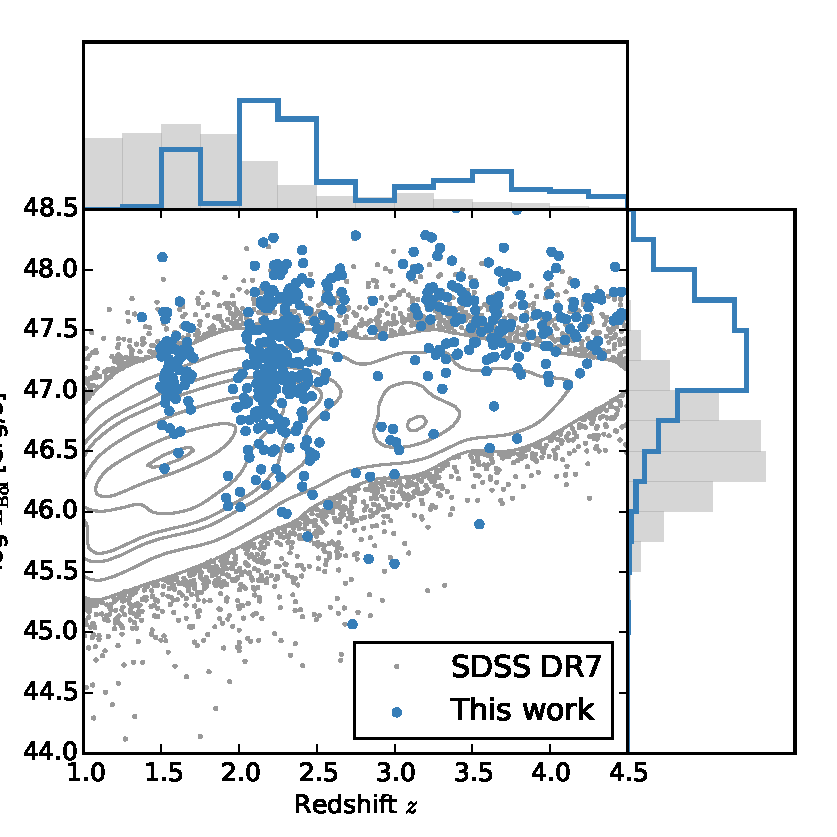
\includegraphics[width=0.8\textwidth]{figures/chapter02/luminosity_z.pdf} 
    \caption[{The redshift and luminosity distribution of our sample.}]{The ranges in redshift and luminosity covered by our sample, relative to the redshift-luminosity distribution of the SDSS DR$7$ quasar catalogue. For the SDSS sample we use \citet{hewett10} redshifts and bolometric luminosities computed by \citet{shen11} from $L(3000\,{\mathrm \AA})$ ($z < 1.9$) and $L(1350\,{\mathrm \AA})$ ($z \gtrsim 1.9$) using bolometric corrections ${\mathrm BC}(3000\,{\mathrm \AA})=5.15$ and $\text{BC}(1350{\mathrm \AA})=3.81$ \citep{richards06}. For the quasars in this work the redshift is defined using the peak of the \hans/\hb emission and the bolometric luminosity is computed from $L(5100\,{\mathrm \AA})$ using $\text{BC}(5100\,{\mathrm \AA})=9.26$ \citep{richards06}.}     
    \label{fig:lzplane}
\end{figure}

In Figure~\ref{fig:lzplane} we show the luminosities and redshifts of the quasar sample relative to the redshift-luminosity distribution of the SDSS DR$7$ spectroscopic quasar catalogue.
Our sample spans a redshift range $1.5 < z < 4.0$ and a bolometric luminosity range $10^{45.5}-10^{48}$\,\ergs. 
Spectra were obtained within one or more of the $JHK$ passbands and the gaps in our sample coverage at $z\sim1.8$ and $z\sim3$ are due to the presence of atmospheric absorption. 
Obtaining near-infrared spectra of adequate resolution and S/N of even moderately bright quasars remains resource intensive. 
As a consequence, at fixed redshift, the luminosities of the quasars are brighter than the average luminosity of the SDSS sample, although the dynamic range in luminosity is a full $1.5$ decades.

\section{Supplementary data}

\begin{table}
  \centering
  \footnotesize 
    \begin{tabular}{ccc}
    \hline
    & Source & \% \\
    \hline
    ($1$) & SDSS & $60$ \\
    ($2$) & BOSS & $45$ \\
    ($3$) & HAMBURG-ESO & $7$ \\
    ($4$) & VLT/UVES & $4$ \\
    ($5$) & VLT/XSHOOTER & $8$ \\ 
    \hline
    \end{tabular}
    \caption[{Percentage of catalogue for which observed-frame optical spectroscopic data is available from the given sources.}]{Percentage of catalogue for which observed-frame optical spectroscopic data is available from the given sources.}
  \label{tab:optical-data}
\end{table} 

\subsection{Observed-frame optical spectroscopic data}

Observed-frame optical spectra are available for $79$ per cent of the catalogue.  
The sources of the optical spectra (summarised in Table~\ref{tab:optical-data}) are as follows:

\begin{enumerate}

 \item SDSS DR$7$ spectroscopic quasar catalogue. Spectra are moderate resolution ($R\simeq2000$) and S/N ($\text{S/N}\simeq20$) and cover the observed-frame wavelength interval $\sim3800-9180$\,\AA.   
 
 \item BOSS DR$12$ \citep{paris17} spectroscopic quasar catalogue. Compared to SDSS spectra, BOSS spectra cover a slightly broader wavelength range and are typically higher S/N. 

 \item The Hamburg-ESO survey \citep{wisotzki00}. The spectra have a typical $R\simeq700$ spectral resolution and S/N $\gtrsim10$ per pixel. 

 \item Spectra taken with VLT/UVES. The reduced and fluxed UVES spectra were made available to us by Dr. A. Dall'Aglio (a description of the reduction procedure is contained in \citealt{dallaglio08}). The spectral resolution of the UVES observations is very high ($R\simeq40\,000$) and the S/N of the spectra, re-binned to a resolution of $R\simeq2000$, is $\text{S/N}\simeq300$. 

 \item Spectra taken with VLT/XSHOOTER. The XSHOOTER spectra are moderate resolution ($R\simeq6000$) and cover the full observed-frame optical-near-infrared spectral region ($0.30-2.50$\,$\mu$m). 

\end{enumerate}

\subsection{Photometric data}

We cross-matched our catalogue with photometric data from a number of wide-field surveys. 
The matching was done using a three arcsecond matching radius, with only the closest neighbour retained in the case of multiple matches. 
The cross-matched surveys and the percentage of successful matches is summarised in Table~\ref{tab:cross-matching}. 
The columns in Table~\ref{tab:cross-matching} are as follows:

\begin{enumerate}

 \item SDSS DR$9$ \citep{ahn12} photometric source catalogue. Point spread function magnitudes. 

 \item Two Micron All Sky Survey \citep[$2$MASS;][]{skrutskie06} Point Source Catalogue. Default magnitudes.

 \item UKIDSS Large Area Survey (DR$10$). One arcsecond radius aperture corrected magnitudes (`apermag$3$').   

 \item Visible and Infrared Survey Telescope for Astronomy (VISTA) Hemisphere Survey \citep[VHS;][]{mcmahon13}. One arcsecond radius aperture corrected magnitudes (`apermag$3$').   

 \item VISTA Kilo-Degree Infrared Galaxy \citep[VIKING;][]{edge13} Survey (DR$4$). One arcsecond radius aperture corrected magnitudes (`apermag$3$').

 \item WISE AllWISE Data Release \citep{mainzer11}. Profile-fitting magnitudes (`mpro').

\end{enumerate}

\subsection{Radio/BAL quasar classification}
\label{sec:ch2-flags}

Using the catalogues provided by \citet{shen11}, \citet{allen11} and \citet{paris17} and visual inspection, 19 quasars in the catalogue are identified as being \ion{C}{IV} BAL quasars.  

We cross-match our catalogue to the FIRST radio catalogue \citep{white97}. 
We classify quasars with matches within five arcsecond as core-dominated, while, if multiple matches are found within $30$\,arcsecond, quasars are classified as lobe-dominated \citep[e.g.][]{shen11}. 
$128$ objects are outside of the FIRST footprint, $269$ are not detected in FIRST, $29$ are detected and are core-dominated, and $8$ are detected and are lobe-dominated. 

\begin{table}
  \centering
  \footnotesize 
    \begin{tabular}{ccccccc} 
    \hline
     & SDSS & $2$MASS & UKIDSS & VHS & VIKING & WISE \\
     & ($1$) & ($2$) & ($3$) & ($4$) & ($5$) & ($6$) \\ 
    \hline
    $u$ & $73$ & - & - & - & - & - \\
    $g$ & $73$ & - & - & - & - & - \\
    $r$ & $73$ & - & - & - & - & - \\
    $i$ & $73$ & - & - & - & - & - \\
    $z$ & $73$ & - & - & - & $9$ & - \\
    $Y$ & - & - & $41$ & $10$ & 9 & - \\
    $J$ & - & $57$ & $41$ & $34$ & $9$ & - \\
    $H$ & - & $57$ & $41$ & $20$ & $9$ & - \\
    $K$ & - & $57$ & $41$ & $33$ & $9$ & - \\
    $W1$ & - & - & - & - & - & $97$ \\
    $W2$ & - & - & - & - & - & $97$ \\
    $W3$ & - & - & - & - & - & $97$ \\
    $W4$ & - & - & - & - & - & $97$ \\
    \hline
    \end{tabular}
    \caption[{Cross-matched surveys and the percentage of successful matches.}]{Cross-matched surveys and the percentage of successful matches.}
  \label{tab:cross-matching}
\end{table} 

\section[Absolute flux calibration]{Absolute flux calibration of near-infrared spectra}

Relative flux-calibration of the infrared spectra as a function of wavelength has been achieved through observations of appropriate flux standards. 
The absolute flux levels, however, can be in error by large factors due to variable atmospheric conditions combined with the narrow slit widths. 
For the majority of the quasars we have, therefore, established the absolute flux scale for each near-infrared spectrum using either SDSS/BOSS spectroscopy or the available photometric data as a fiducial baseline.
The methods are attempted in the order given below, and the method we adopt is dependent on the availability of the required data. 
We are unable to verify the absolute flux calibration of the near-infrared spectra for four objects because neither SDSS/BOSS spectra nor optical/near-infrared data is available. 
The methods used to flux calibrate the near-infrared spectra are summarised in Table~\ref{tab:flux_calibration}. 

\subsection{SDSS spectrum as a fiducial baseline}

The flux calibration of the SDSS spectra is excellent, and so these spectra can be used as a fiducial baseline to calibrate the near-infrared spectra. 
The quasar SED model described in Chapter~\ref{ch:sed} is used to bridge the gap between the wavelength coverage of the near-infrared and optical SDSS spectrum.
This model provides a very good fit to the SDSS and UKIDSS magnitudes of SDSS DR$7$ quasars, reproducing the individual magnitudes to $<0.1$\,mag.
The first step is to normalise the SED model to the SDSS spectrum. 
This is done using a variance-weighted $\chi^2$ minimisation procedure in several emission-line-free intervals of the spectrum.   
The second step is to normalise the near-infrared spectrum to the SED model. 
Again, this is done using a variance-weighted $\chi^2$ minimisation procedure, with regions of the spectrum falling between the near-infrared passbands masked-out in the minimisation. 
The flux calibration procedure is demonstrated in Figure~\ref{fig:normalise_to_sdss_a}. 

\subsection{BOSS spectrum as a fiducial baseline}

This procedure is identical to one described in the previous section, the only difference being that the SDSS spectrum is substituted for a BOSS spectrum. 
To avoid the known issues in the flux calibration of the BOSS DR$12$ quasar spectra at observed-frame blue wavelengths \citep{lee13}, our fitting was confined to rest-frame wavelengths long-ward of $1275$\,\AA.

\begin{figure}
    \captionsetup[subfigure]{labelformat=empty}
    \centering
    \subfloat[\label{fig:normalise_to_sdss_a}]{}
    \subfloat[\label{fig:normalise_to_sdss_b}]{}    
    \subfloat[]{{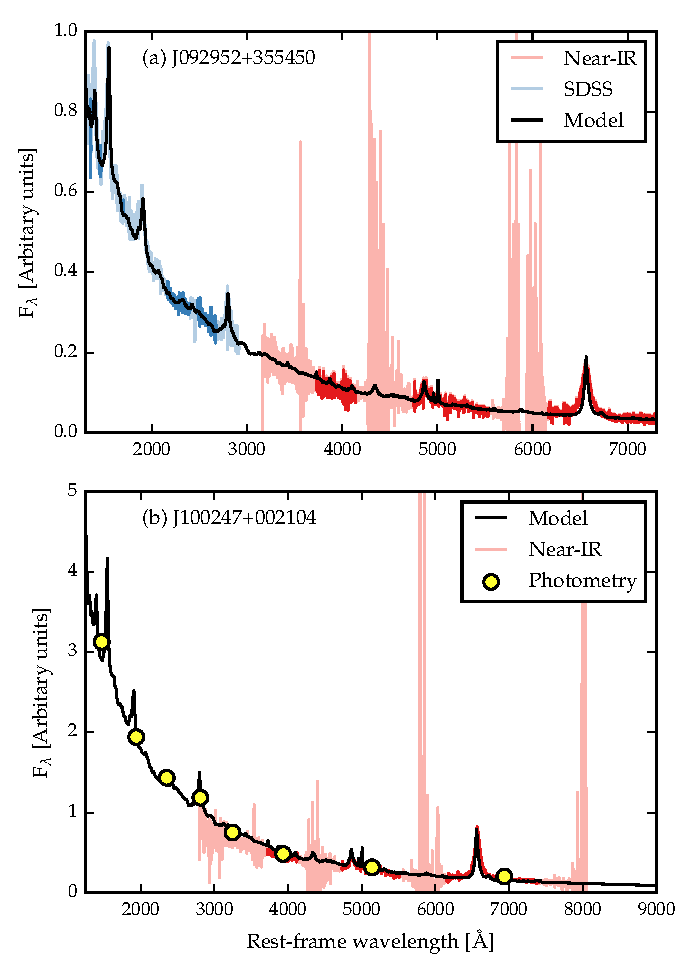
\includegraphics[width=\textwidth]{figures/chapter02/normalise_to_sdss.pdf} }}
    \caption[{Demonstration of how the absolute flux calibration of a near-infrared spectrum is established.}]{Demonstration of how the absolute flux calibration of a near-infrared spectrum is established using the SDSS spectrum (a) or photometric data (b) as fiducial baselines. An empirical quasar SED model is used to bridge the discontinuity in the wavelength coverage of the optical/near-infrared spectroscopic and photometric data. The darker regions of the spectra are used in the fitting procedures.}     
    \label{fig:normalise_to_sdss}
\end{figure}

\subsection{Photometric data as a fiducial baseline}

In the first step, the quasar SED model is normalised to the available optical (SDSS) and near-infrared (VHS, Viking, UKIDSS or $2$MASS) photometric data. 
The SED model is integrated through the appropriate passband transmission functions to give model magnitudes (Equations~\ref{eq:flux} and \ref{eq:mag}), and a variance weighted $\chi^2$ minimisation procedure is performed with the observed magnitudes.
The second step in the procedure is then identical to the previous two sections.   
This procedure is illustrated in Figure~\ref{fig:normalise_to_sdss_b}. 

\begin{table}
  \centering
  \footnotesize 
    \begin{tabular}{cc} 
    \hline
    Method & \% \\
    \hline
    SDSS               & $60$ \\
    BOSS               & $9$ \\
    NIR photometry     & $25$ \\
    NIR+OPT photometry & $6$ \\
    None               & $1$ \\    
    \hline
    \end{tabular}
    \caption[{Methods used in absolute flux calibration of near-infrared spectra.}]{Methods used in absolute flux calibration of near-infrared spectra.}
  \label{tab:flux_calibration}
\end{table} 

\subsection{Reliability of luminosity measurements}

The fluxes at $1350$ and $5100$\,\AA\, were read off directly from the normalised SED model. 
These were converted into monochromatic continuum luminosities, which are used to compute BH masses and bolometric luminosities in Chapters~\ref{ch:bhmass}, \ref{ch:nlr} and \ref{ch:sed}. 
Comparison of the $5100$\,\AA\, luminosity, computed using the photometry- and spectrum-based methods for $296$ quasars, showed a scatter (mean absolute deviation) of just $\sim0.1$\,dex.
We therefore assume $0.1$\,dex to be the measurement uncertainty on the $5100$\,\AA\, luminosities.
We expect the uncertainties on the $1350$\,\AA\, luminosities to be at similar level.  
For all the catalogue quasars, the optical and near-infrared spectra as well as the near-infrared photometry were obtained at different epochs, with rest-frame time differences of up to $\sim5$ years. 
Intrinsic quasar photometric variability in the rest-frame ultra-violet and optical will therefore add additional scatter of $\sim0.2$\,mag \citep[e.g.][]{macleod10} to the derived $1350$ and $5100$\,\AA\, luminosities.

The monochromatic continuum luminosity at $5$\,$\mu$m was also computed by linearly interpolating through the WISE photometric data points. 
$5$\,$\mu$m luminosities were derived in this way for $434$ quasars up to redshift $z=3.4$. 
At higher redshifts, the longest wavelength WISE passband ($W4$) is at $<5$\,$\mu$m in the quasar rest-frame and so $5$\,$\mu$m luminosities could not be computed using this method.

\section[Instrumental broadening]{Correcting for instrumental broadening}

\begin{table}
  \centering
  \footnotesize 
    \begin{tabular}{cc} 
    \hline
    Spectrograph & FWHM [\kms] \\
    \hline
    FIRE         & $59$ \\
    GNIRS        & $136$ \\
    ISAAC        & $46$ \\
    LIRIS        & $477$ \\
    NIRI         & $465$ \\
    NIRSPEC      & $122$ \\
    SINFONI      & $124$ \\
    SOFI (MR)    & $323$ \\
    SOFI (LR)    & $535$ \\
    P200 TRIPLESPEC & $88$ \\
    ARC TRIPLESPEC  & $97$ \\
    XSHOOTER     & $25$ \\
    SDSS/BOSS & $152$ \\
    UVES & $3$ \\
    HAMBURG-ESO & $400$ \\
    \hline
    \end{tabular}
    \caption[{Spectral resolutions of the spectrographs used in this thesis.}]{Spectral resolutions of the spectrographs used in this thesis.}
  \label{tab:specres}
\end{table} 

Throughout this thesis, reported line-width measures are corrected for instrumental broadening by subtracting the resolution of the spectrograph in quadrature. 
Because the quasar emission-line profiles are typically non-Gaussian, this deconvolution procedure is only approximate. 
The spectrograph resolutions, which we estimate from the line widths in the observed sky spectra, are given in Table~\ref{tab:specres}. 
The resolutions are generally small relative to the widths of quasar broad emission-lines (FWHM $\sim4000$\,\kms).  

